\section{Simulation}

In order to test \acrshort{ldr}'s performance and compare it with the lightning network's current routing solution, a payment routing simulator was developed \cite{simulator}. \\
Using as its underlying network a snapshot of the real lighting network, the simulator is able to reproduce payments between different pairs of nodes using different routing schemes. To define the initial states of channels with capacity C, and since the state channel information of third party nodes is not public, all channels between two nodes A and B are initialized with the state (A: $\frac{C}{2}$, B: $\frac{C}{2}$). Lastly, and since they are not the focus of the study done by the simulation, the channel routing fee's are not contemplated by it.\\

The simulation has the following parameters:
\begin{itemize}
    \item Number of payments
    \item Number of nodes
    \item Mean weight
    \item Variance weight
\end{itemize}
The parameter that defines the number of nodes to be removed is used to control the size of the network, opening the possibility of making it smaller and thus easier to run simulations on. Nodes are removed randomly but as a result of working with a scale-free network there is an inherited robustness \cite{network_science} which reduces the resulting fragmentation to a minimum, a phenomenon that is studied in \cite{ln_topological}. When the network is fragmented as a result of the removal of nodes all the connected components but the one with the most nodes are removed so the simulation can run on a one component graph.\\
$P$, the random variable that represents the amount for each payment, follows a normal distribution with free $(\mu,\,\sigma^{2})$ parameters. Both these parameters are determined using equations \ref{eq:distribution_mu} and \ref{eq:distribution_sigma}. 
\begin{equation}
    \mu = Mean weight * Median Channel Balance
    \label{eq:distribution_mu}
\end{equation}
\begin{equation}
    \sigma = Variance weight * Median Channel Balance
    \label{eq:distribution_sigma}
\end{equation}
\\
There is also a parameter associated with \acrshort{ldr}:
\begin{itemize}
    \item Number of routing gossip messages between payments
\end{itemize}
It's important to properly set the number of routing message exchanges between each payment since this parameter will define how well the routing tables present in each node can adapt to the dynamics of the network.\\
The number of entries associated with each destination in \acrshort{ldr} is kept at one by the simulation so the memory requirements of the simulation are kept low.\\
The current source routing solution based on Dijkstra's shortest path algorithm has no free parameters.\\

After some testing with the simulator parameters were set to the ones in table \ref{table:simulation_params1}. 200 payments were enough to obtain steady results, with the addition of more payments not resulting in clear output changes. The number of nodes was chosen so that the resulting networks could be big enough to be significant but no so big such that it slowed down the simulation beyond acceptable levels, resulting networks end up
on the order of dozens of nodes. The number of gossip messages was set to 10 on the belief that on a real network there would be at least an order of magnitude more gossip messages than payments. Mean and variance weights were set to start low so payment volumes will be low and increase the chance of success for payments with the variance being half of the mean so the distribution is acceptably spread out.

\begin{table}[H]
\centering
\resizebox{\columnwidth}{!}{\begin{tabular}{|l|l|l|l|l|}
\hline
\rowcolor[HTML]{C0C0C0} 
\# Payments & \# Nodes to remove & Mean weight & Variance weight & \# Gossip Messages\\ \hline
200 & 280 & 0.1 & 0.05 & 10\\ \hline
\end{tabular}}
\label{table:simulation_params1}
\end{table}

After it goes through the node removal and address assignment processes the simulation returns figure \ref{fig:sim_net_addr}, an image representation of the network that will be used to simulate on.

\begin{figure}[H]
\begin{center}
  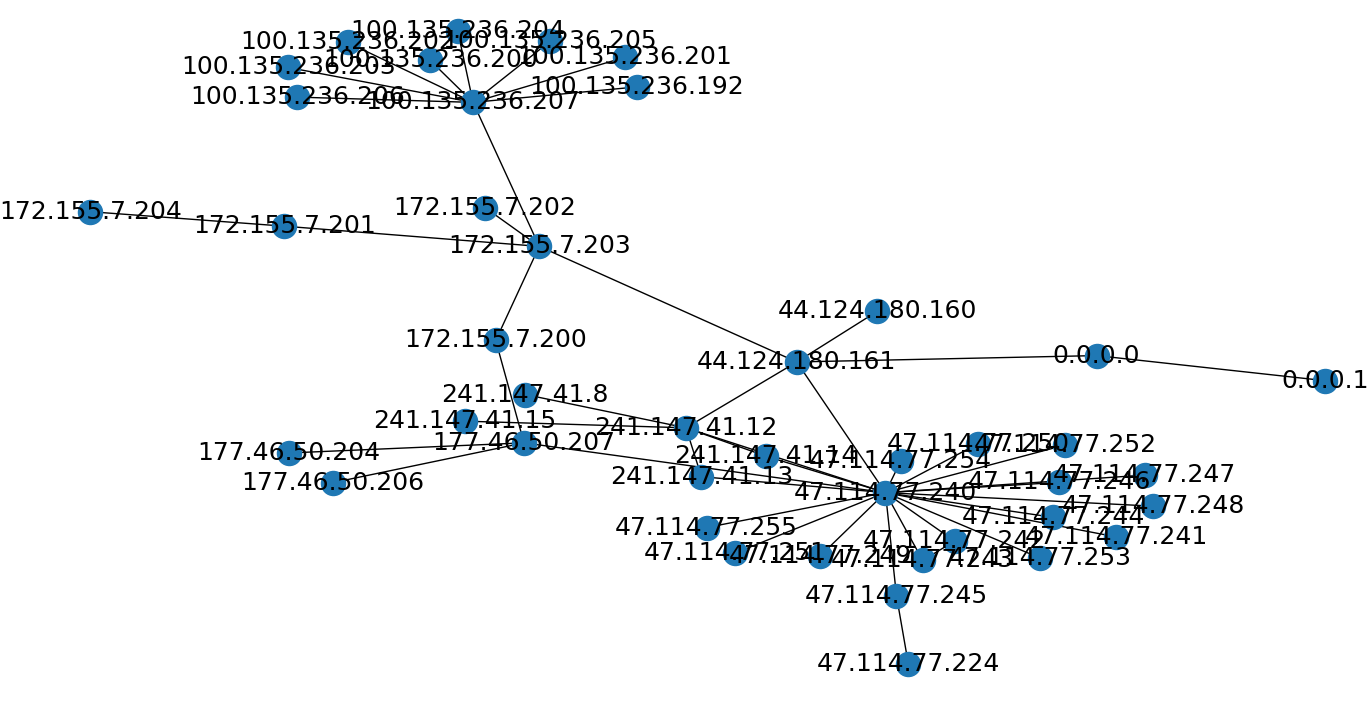
\includegraphics[width=\linewidth]{images/sim_net_addr.png}
  \caption{Network after address issuing}
  \label{fig:sim_net_addr}
  \end{center}
\end{figure}

The design of the address validation rules aims to promote a healthy network through similar addressing of nodes who are close together. The results of this effort are very noticeable in the network in figure \ref{fig:sim_net_addr} where there are various clusters of nodes who share addresses that are close in the address space. Nodes belonging to subnetworks 100.135.236.0/24, 172.155.7.0/24 and 47.114.77.0/24 can be found clustered together.\\
In the end, the simulation returned the routing metrics found in table \ref{table:simulation_results1}.

\begin{table}[H]
\centering
\begin{tabular}{l|l|l|}
\cline{2-3}
\rowcolor[HTML]{C0C0C0} 
\cellcolor[HTML]{FFFFFF}                  & SPR     & LDR    \\ \hline
\multicolumn{1}{|l|}{P(Success)}          & 61.0\%  & 61.5\% \\ \hline
\multicolumn{1}{|l|}{P(Overcap|Failed)}   & 100.0\% & 97.4\% \\ \hline
\multicolumn{1}{|l|}{P(NonExis|Failed)}   & 0.0\%   & 2.6\%  \\ \hline
\multicolumn{1}{|l|}{\acrshort{apl}} & 3.56    & 3.75   \\ \hline
\end{tabular}
\caption{Results for the first simulation}
\label{table:simulation_results1}
\end{table}

Results show little difference between the probability of payment success of the new routing solution (\acrshort{ldr}) and the current Dijkstra's \acrfull{spr} algorithm. This is due to the fact that, in this case, most of the payments' volumes are small compared to the balances available in the channels to "push" the payment to the next node. Meaning that almost every path, including the shortest one, will be able to route the payment without any balance constraints. The fact that almost every path from node A to B can be used to send a payment through makes the advantages of using \acrshort{ldr} over the current solution negligible. Payment errors due to lack of channel balance, the biggest issue tackled by \acrshort{ldr}, are rare when payment volumes are low.\\
The simulation gives some insight on the how payments fail, these can happen in one of two ways; because the payment's volume is bigger than one of the routes' channels balances or because a route to the destination was not found, $P(Overcap|Failed)$ and $P(NonExis|Failed)$ respectively. Since we are always simulating on a connected graph, Dijkstra's shortest path algorithm will always find a path between two nodes and \acrshort{spr}'s $P(NonExis|Failed)$ will always be 0\%.\\
The \acrfull{apl} is bigger when using \acrshort{ldr}. This is expected because, unlike what happens with \acrshort{spr}, \acrshort{ldr} does not always choose the shortest path to the destination.

\begin{table}[H]
\centering
\resizebox{\columnwidth}{!}{\begin{tabular}{|l|l|l|}
\hline
\rowcolor[HTML]{C0C0C0} 
{\color[HTML]{000000} Median Channel Balance} & {\color[HTML]{000000} Payment's Distribution $\mu$} & {\color[HTML]{000000} Payment's Distribution $\sigma$} \\ \hline
500000                                        & 50000                    & 2500                     \\ \hline
\end{tabular}}
\caption{Median channel balance and payment volume distribution parameters}
\label{table:simulation_channel_info1}
\end{table}

Table \ref{table:simulation_channel_info1} confirms that the median value of the channels' balances distribution is an order of magnitude larger than the payment's distribution $\mu$, making the channels' balances much bigger than the payment volumes and the \acrshort{ldr}'s advantages over the current implementation negligible. \\

In order to have a better insight on how the difference in probability of success changes changes with the size of the payment's volume every parameter in table \ref{table:simulation_params1} was kept, with the exception of the mean and variance weights. Then the simulation was repeated 100 times for each of the different (MeanWeight, VarianceWeight) pair.
The mean weight was then varied and the variance weight calculated as its function according to equation \ref{eq:variance_calc}.
\begin{equation}
    Variance weight = \frac{Mean weight}{2}
    \label{eq:variance_calc}
\end{equation}
And $\overline{\Delta}$ defined as:
\begin{equation}
    \overline{\Delta} = \overline{P(Success)_{LDR}} - \overline{P(Success)_{SPR}}
\end{equation}

Figure \ref{fig:simulation_results4} portrays the result of the simulations.

\begin{figure}[H]
\begin{center}
  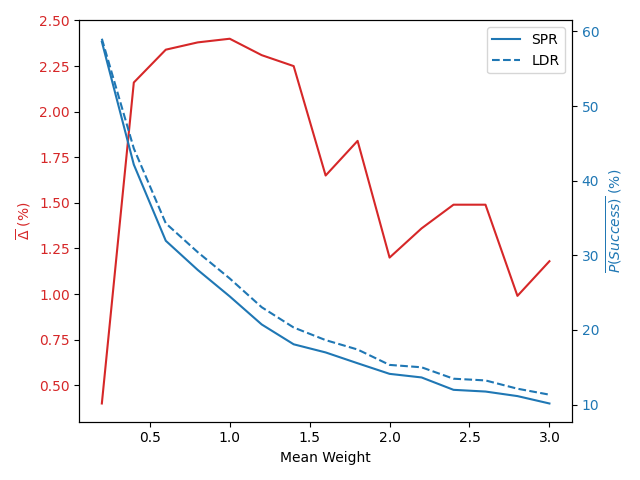
\includegraphics[width=\linewidth]{images/simulation_results4.png}
  \caption{$\overline{\Delta}$ and  $\overline{P(Success)}$ as a function of the mean weight}
  \label{fig:simulation_results4}
  \end{center}
\end{figure}

As the mean weight and consequently the payments' volumes increase there is also an increase in the value of $\overline{\Delta}$, restating the conclusion that \acrshort{ldr}'s advantage over the current implementation gets larger as the payments' volumes increase. This only happens up to a certain point though, after reaching a maximum the $\overline{\Delta}$ value starts falling. The reason for this is that, since payments are getting bigger, the probability that the number of possible paths between two nodes that support such voluminous payments starts decreasing, a fact supported by the decrease in the average P(Success) for both solutions and that ends up diminishing \acrshort{ldr}'s advantage of being able to route through bigger capacity paths because not even those are able to support the increasingly bigger volumes.\\
Lastly, the effects of increasing the underlying network of the simulation were studied through the increase of the "Number of nodes" parameter while keeping the rest of table's \ref{table:simulation_params1} parametrization. Up to this point, all simulations were run with networks that were reduced to 280 nodes before the biggest component was chosen to be the base network of the simulation. Increasing the number of nodes the network is reduced to will increase the size of the biggest component and base network of the simulation. This also increases its running time due to the fact that each simulated node stores a routing table that can have information about each one of the other nodes, forming a performance quadratic upper bound, $\mathcal{O}(n^2)$.\\
To solve this issue the number of simulations was scaled down from 100 to 10. The results are given by figure \ref{fig:simulation_results5}.\\

\begin{figure}[H]
\begin{center}
  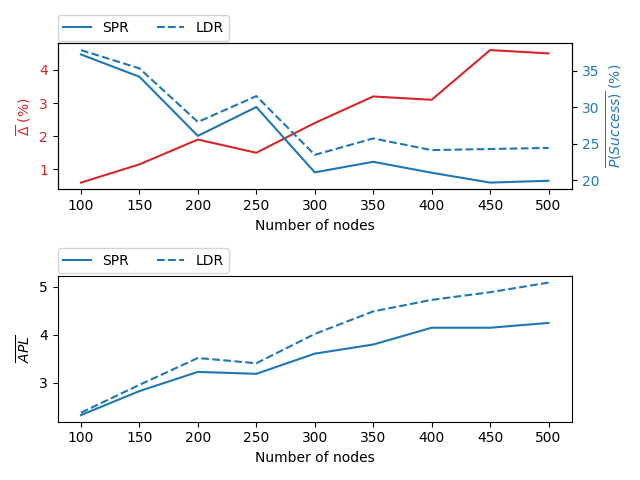
\includegraphics[width=\linewidth]{images/simulation_results5.png}
  \caption{$\overline{\Delta}$, $\overline{P(Success)}$ and \acrshort{apl} as a function of the number of nodes}
  \label{fig:simulation_results5}
  \end{center}
\end{figure}

As the number of nodes increases the advantage of using \acrshort{ldr} over \acrshort{spr}, represented by their performance difference $\overline{\Delta}$, also increases. This behaviour can be explained by two consequences of adding new nodes:
\begin{enumerate}
	\item The \acrshort{spr}'s \acrshort{apl} increases, which means payment paths will be longer and there will be more opportunities for an \acrshort{spr} payment to fail due to capacity constraints.
	\item Every new node added to the network creates a new opportunity for an \acrshort{ldr} node to adapt its paths through it, possibly creating bigger capacity routes than the ones that were available before.
\end{enumerate}

As can already be noticed in figure \ref{fig:simulation_results5} the increase in \acrshort{spr}'s \acrshort{apl}, as a function of the number of nodes, slows down. In fact, when approximating the \acrshort{spr}'s \acrshort{apl} for the entire network with 4420 nodes the result was:
 \begin{equation}
     \acrshort{apl} = 4.65
\label{eq:ln_apl}
 \end{equation}
 The result obtained in equation \ref{eq:ln_apl} was calculated by averaging the \acrshort{spr}'s \acrshort{apl} between $n$ pairs of random nodes, with $n=10000$ and its result corroborates the fact that \acrshort{spr}'s \acrshort{apl} growth slows down. Subsequently, and as networks get bigger, increases in $\overline{\Delta}$ will not rely on an increase in \acrshort{spr}'s. Instead, they will mostly rely on how well \acrshort{ldr} can adapt its payment paths and maximize their capacity.\\ 